%Folgende Zeile aktivieren und als SVN property "svn:keywords" auf "Id" setzen, um SVN Versionsinformationen im Dokument zu erhalten
%\svnInfo $Id: einleitung.tex 60 2012-01-26 15:56:06Z koppor $ 

\chapter{2D - Verfahren}
\label{chap:2d}
	\section{SIFT}
		SIFT (Scale-invariant feature transform) ist ein von David Lowe 1999 vorgestelltes Verfahren zur Extraktion von lokalen Merkmalen aus Bildern. Die mit diesem Verfahren gefundene Merkmale haben die Eingeschaft, dass sie robust gegenüber Rotation, Translation und Skalierung sind, und damit zuverlässig in anderen Bilder wiedererkannt werden können.
Um Objekte in Bildern mit SIFT erkennen und lokalisieren zu können, sind also zwei Schritte nötig:
\begin{enumerate}
	\item Extraktion und Beschreibung von Merkmalen (Features) des gesuchten Objekts
	\item Lokalisation der Merkmale im Suchbild
\end{enumerate}

\subsection{Extraktion und Beschreibung von Merkmalen (Features) des gesuchten Objekts}
Der Algorithmus zur Extraktion und Beschreibung der Merkmale besteht dabei aus vier Verarbeitungsstufen:
	\subsubsection{Ermittlung potentieller Merkmale in DoG-Pyramiden}
		Um Merkmale zu ermitteln, die robust gegenüber Skalierung sind, kommt das Verfahren der DoG (Difference of gaussians) Pyramiden zum Einsatz. Dabei werden aus dem Ausgangsbild zunächst n Gaußpyramiden berechnet. Eine Pyramide besteht dabei aus fortlaufen stärker geglätteten Bildern des Ausgangsbildes $g$. Zur Glättung kommt dabei ein Gaußfilter $G$ zum Einsatz:
\begin{equation*}
 g(x, y) * G_\vartheta (x, y) = g(x, y) * (\frac{1}{\sqrt{2\pi \vartheta ^2}}\cdot e^{-\frac{x^2 + y^2}{2\vartheta ^2}})
\end{equation*}

Im Anschluss wird das letzte Bild der Pyramide um 50\% verkleinert, und daraus durch erneute fortlaufende Glättung mit dem Gaußfilter eine neue Pyramide erzeugt.
Je zwei benachbarte Bilder einer Gaußpyramide werden nun voneinander Subtrahiert. Aus den Resultaten entstehen dabei die DoG Pyramiden:
\begin{figure}
  \begin{center}
    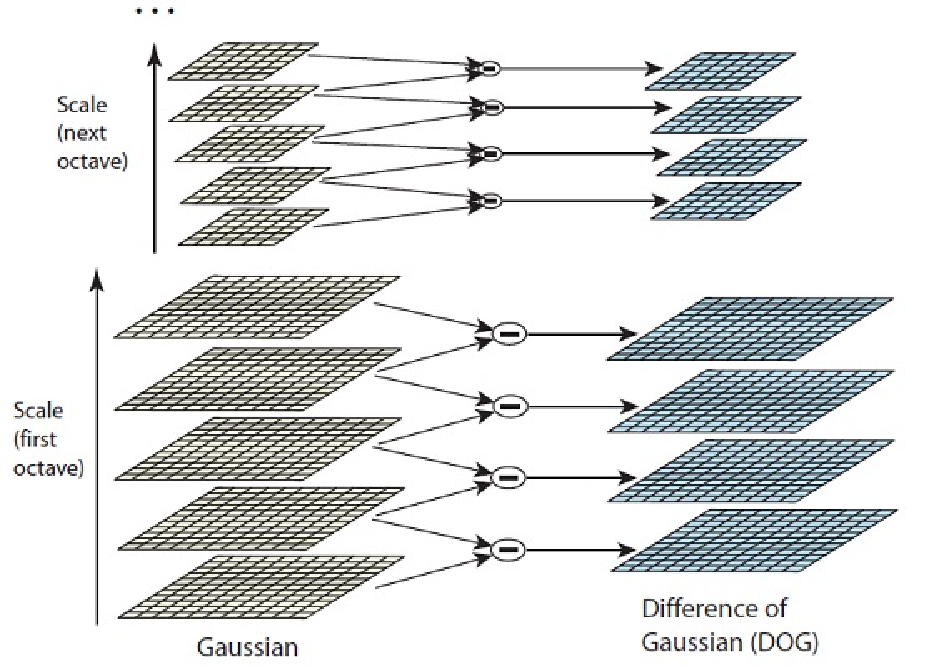
\includegraphics[width=\textwidth]{dog.pdf}
    \caption{DoG-Pyramiden}
    \label{fig:dog_pyr}
  \end{center}
\end{figure}

Die dadurch erzeugten DoG-Pyramiden werden nun auf minimale und maximale Pixelwerte untersucht.
Ein Maximum ist gefunden, wenn der Grauwert eines Pixels größer als der seiner 26 Nachbarn ist. Nachbarschaft eines Pixels ergibt sich dann aus seinen acht Nachbarn der selben Ebene, sowie aus den jeweils neun Nachbarn der benachbarten Ebenen in der DoG-Pyramide.
Die Suche nach Minima erfolg auf die selbe Art und Weise. Die Information, auf welcher Skalierung die potentiellen Merkmalspunkte liegen, wird dabei ebenfalls gespeichert.
\begin{figure}[H]
  \begin{center}
    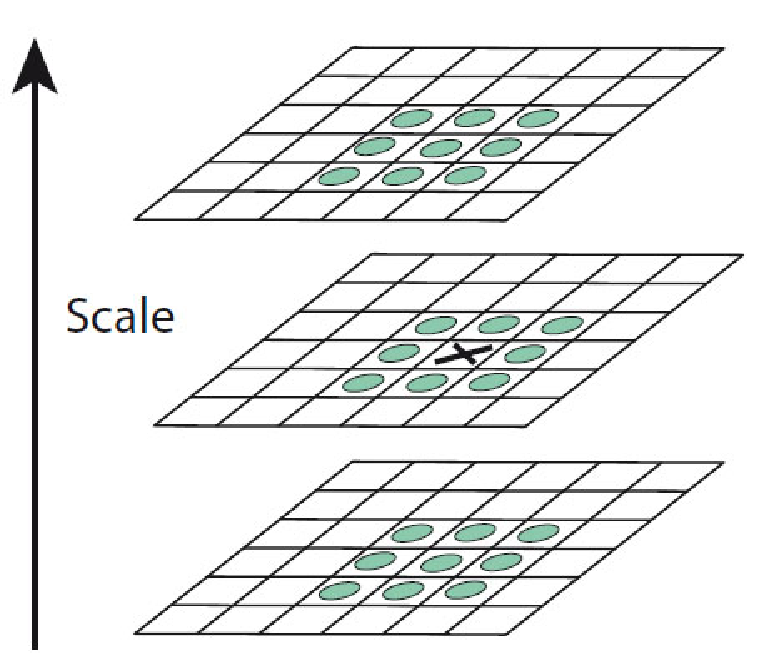
\includegraphics[width=0.5\textwidth]{scale.pdf}
    \caption{Nachbarschaft eines Pixels}
    \label{fig:neighbor}
  \end{center}
\end{figure}
	\subsubsection{Filterung und Lokalisation potentieller Merkmalspunkte}
		Das oben genannte Verfahren liefert neben den robusten Merkmalspunkten eine große Menge von instabilen, für die weitere Verarbeitung nicht zu gebrauchende Merkmale.
Daher werden die gefundenen Merkmalspunkte anhand von Stabilitätskriterien gefiltert.
Im ersten Schritt werden dabei alle Merkmalspunkte entfernt, die einen DoG-Wert von weniger als 0,03, und somit einen relativ niedrigen Kontrast besitzen.
Merkmalspunkte, die auf Ecken liegen sind “prägnanter” (und somit staibler) als solche, die auf einer Kante liegen, daher werden alle Merkmalspunkte entfernt, die auf einer Kante, aber nicht auf einer Ecke liegen.
Dies geschieht unter Anwendung der Hesse-Matrix (todo).
	\subsubsection{Bestimmung der Hauptorientierungen}
		Um Invarianz der verbleibenden Merkmalspunkte gegenüber Rotation zu erreichen, wird für jeden Merkmalspunkt dessen Hauptorientierung berechnet.
Dafür nutzt man das gaußgefilterte Bild, welches der Skalierung des zu untersuchenden Merkmalspunktes am nächsten kommt. In diesem Bild werden nun innerhalb einer festen Region um den Merkmalspunkt herum die Gradientenlängen $m(x, y)$ und die Gradientenorientierungen $\theta (x, y)$ bezüglich eines Punktes $g(x, y)$ berechnet, wobei
\begin{equation*}
m(x, y) = \sqrt{(g(x + 1, y) - g(x - 1, y))^2 +(g(x, y+1) - g(x, y-1))^2}
\end{equation*}

und

\begin{equation*}
\theta (x, y) = tan^{-1}\cdot \frac{g(x +1, y) - g(x-1, y)}{g(x, y +1) - g(x, y-1)}
\end{equation*}

Die so ermittelten Gradientenorientierungen werden nun anhand ihrer Gradientenlängen gewichtet. Dadurch haben Gradientenrichtungen mit großer Gradientenlänge einen größeren Einfluss auf die Hauptorientierung als Gradientenrichtungen mit niedriger Gradientenlänge.
Danach werden die Gradientenorientierungen zusätzlich anhand ihrer Entfernung zum Merkmalspunkt gewichtet, um Gradientenrichtungen, die sich näher am Merkmalspunkt befinden stärker zu gewichten.

Aus den gewichteten Gradientenorientierungen wird nun ein Orientierungshistogramm erstellt. Dieses Histogramm ist in 36 Winkelbereiche eingeteilt und hat somit eine Klassenbreite von $10\,^{\circ}$.
Jede Gradientenorientierung wird dabei anhand ihrer Gewichtung an der passenden Stelle im Histogramm aufaddiert. \\
Nach der Erstellung des Histogramms kann aus diesem die Gradientenlänge $m_{max}$ abgelesen werden (Winkelbereich mit der größten Summe). Die Hauptorientierung des Merkmalspunktes  setzt sich dabei aus $m_{max}$, sowie der zugehörigen Gradientenorientierung $\theta_{max}$ maxzusammen.
Für den Fall, dass eine weitere Orientierung mit der Gradientenlänge $m_i > 0,8 m_{max}$
existiert; wie es bei Eckpunkten häufig der Fall ist; wird an der Stelle $(x, y)$ ein weiterer Merkmalspunkt mit der Hauptorientierung $(m_i, \theta_i)$ erstellt.
\subsection{Lokalisation der Merkmale im Suchbild}
Wurden nun im ersten Schritt die robusten Merkmale des gesuchten Objekts extrahiert, können diese im Suchbild wiedererkannt werden.
Dies geschieht, in dem man die extrahierten Merkmale des Objekts mit denen im Suchbild auf Übereinstimmung hin untersucht.
Dafür existieren verschiedene Ansätze.
	\subsubsection{Merkmalsvergleich anhand des eukllidischen Abstands}
Der einfachste Ansatz zwei Deskriptoren miteinander zu Vergleichen, ist die Bestimmung des euklidischen Abstands der Merkmalsvektoren
\begin{equation*}
e = \sqrt{\sum_{i = 1}^{n}(V_{1i} - V_{2i})}
\end{equation*}

\section{Einsatz von SURF zur Erkennung von Bohrpunkten}
Um in den Beispieldatensätzen Bohrpunkte auf möglichst effiziente Art und Weise erkennen zu können, wird hier SURF ($Speeded Up Robust Features$), eine leicht veränderte Variante des SIFT-Verfahrens, verwendet. \\
Der Unterschied zum hier vorgestellen SUFT Verfahrens besteht darin, dass statt der Gaußfilter Mittelwertfilter zum Einsatz kommen. Dadurch wird das Verfahren signifikant beschleunigt, ohne die Erkennungsrate nennenswert zu beeinflussen. \cite{Bay2005} \\

Um Bohrpunkte mithilfe des SURF Verfahrens zu detektieren, wird zunächst ein Modell des Bohrpunktes auf dessen Merkmale hin untersucht. Dazu wird ein Template eines Bohrpunktes aus einem Bild im Bilderstack ausgeschnitten.
\begin{figure}[H]
  \begin{center}
    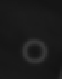
\includegraphics[width=0.4\textwidth]{sift_template.pdf}
    \caption{Modell eines Bohrpunktes (Vergrößert)}
    \label{fig:sift_template}
  \end{center}
\end{figure}


Auf dieses Template wird nun der besprochene SURF Algorithmus angewandt, um die Merkmalsvektoren des Bohrpunktes zu extrahieren.
Das Template wurde dabei bewusst so klein gewählt, dass das Verfahren genau einen Merkmalsvektor liefert, welcher den Bohrpunkt repräsentiert:
\begin{figure}[H]
  \begin{center}
    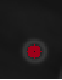
\includegraphics[width=0.4\textwidth]{template_merkmal.pdf}
    \caption{Bohrpunkt mit eingezeichnetem Merkmalsvektor (Vergrößert)}
    \label{fig:template_merkmal}
  \end{center}
\end{figure}

Im nächsten Schritt werden die Merkmalsvektoren im Suchbild extrahiert, wobei wieder der SURF-Algorithmus zum Einsatz kommt, und eine Liste mit Merkmalsvektoren liefert. Zur Illustration werden auch hier die Orte der Merkmalsvektoren in das Suchbild gezeichnet:
\begin{figure}[H]
  \begin{center}
    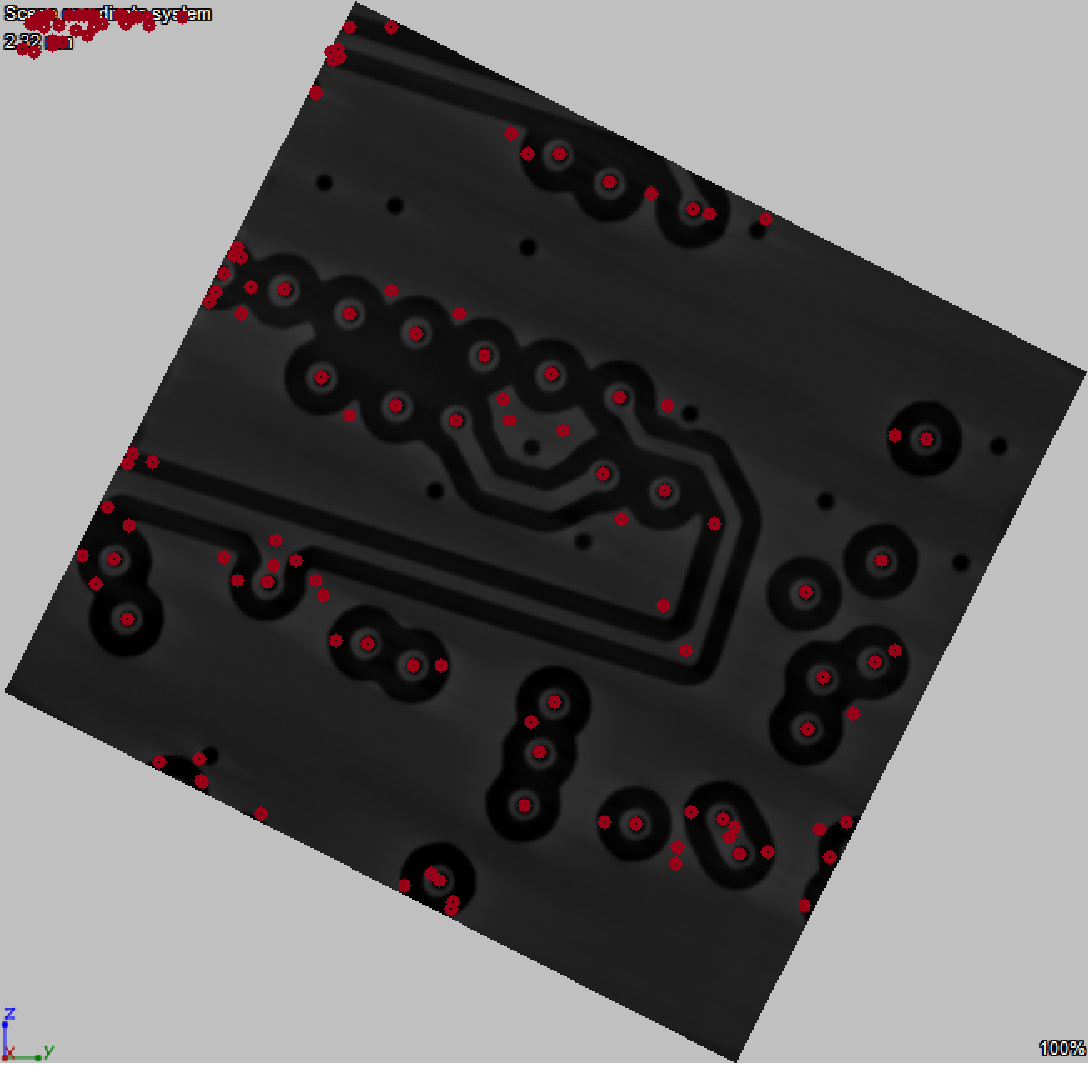
\includegraphics[width=0.8\textwidth]{keypoints.pdf}
    \caption{Suchbild mit eingezeichneten Merkmalsvektoren}
    \label{fig:suchbild_merkmal}
  \end{center}
\end{figure}

Anschließend wird für den Merkmalsvektor des Templates nach Übereinstimmungen in der Liste der Merkmalsvektoren des Suchbildes gesucht, d.h. es wird nach Merkmalsvektoren gesucht, die dem des Templates möglichst ähnlich sind. Ähnlich bedeutet hier, dass die Komponenten zweier Merkmalsvektoren eine hohe Übereinstimmung haben, was genau dann der Fall ist, wenn beide Merkmalsvektoren einen geringen Abstand im Merkmalsraum haben. \\
Daher wird der euklidische Abstand des Merkmalsvektors des Templates mit jedem Merkmalsvektor der Liste berechnet. Ist der Abstand dabei kleiner als $0,45$ im Merkmalsraum, wird eine Übereinstimmung der beiden Merkmalsvektoren angenommen.\\
Dabei werden folgende übereinstimmende Merkmalsvektoren gefunden:
\begin{figure}[H]
  \begin{center}
    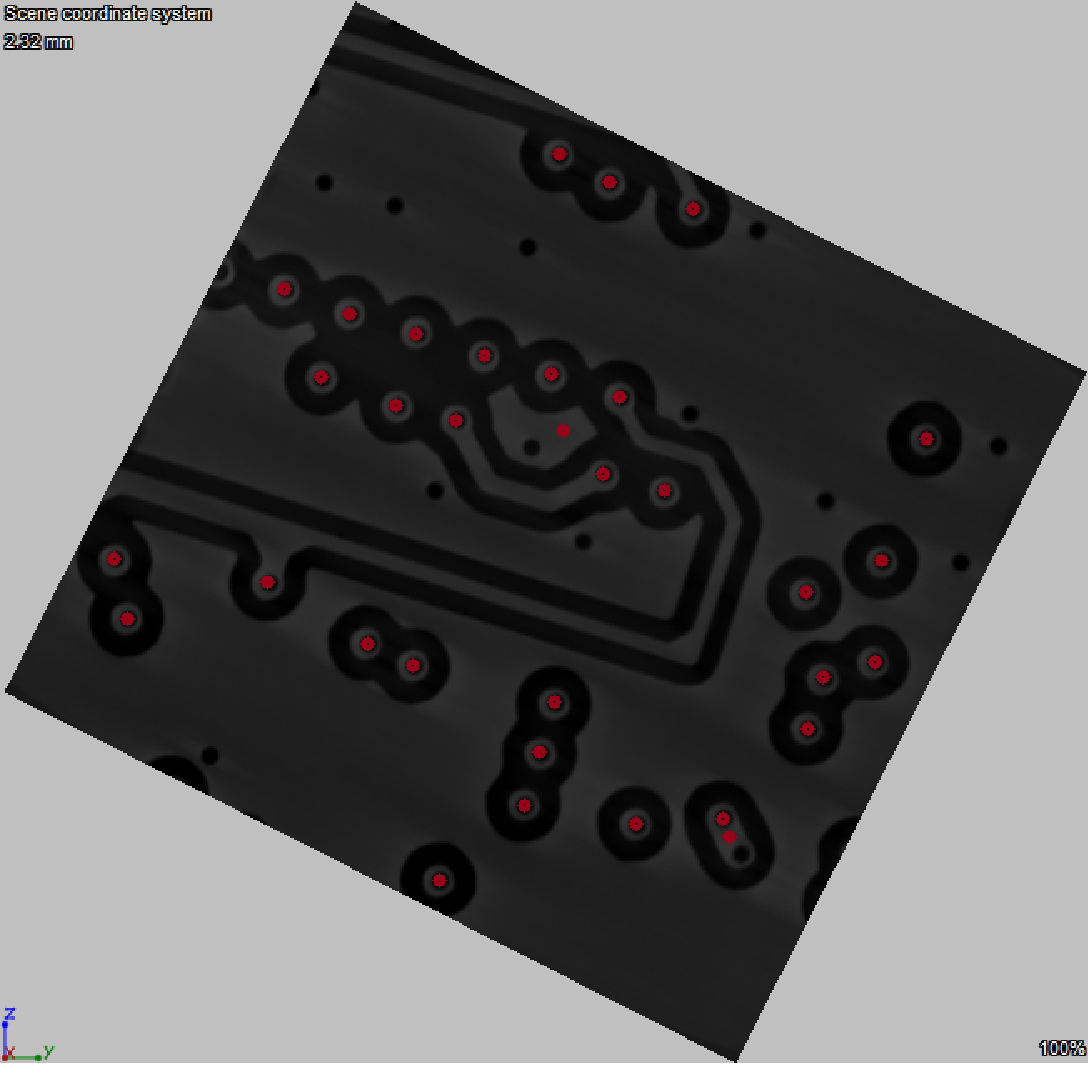
\includegraphics[width=0.8\textwidth]{matches.pdf}
    \caption{Suchbild mit eingezeichneten übereinstimmenden Merkmalsvektoren}
    \label{fig:suchbild_merkmal_matches}
  \end{center}
\end{figure}

Wie deutlich zu sehen ist, werden Borpunkte, die visuell dem Template entsprechen (Bohrpunkt mit äußerer Isolierschicht) fehlerfrei erkannt. Allerdings werden die Bohrpunkte ohne isolierschicht nicht erkannt. Dieser Umstand lässt sich durch eine Modifikation des Suchverfahrens verbessern.

\section{Erweiterung der Merkmalssuche}

Wie im vorigen Abschnitt gezeigt wurde, erkennt das Verfahren des Matchings mit von SIFT-Merkmalen bei einem einzelnen Bild nicht zufriedenstellend, da die Merkmale der Bohrpunkte ohne Isolierschicht nicht eine zu große Distanz zum Merkmalsvektor des Templates im Merkmalsraum haben. \\
Allerdings zeigt sich, dass in Bilder, die sich im Bilderstack nahe am im vorigen Kapitel untersuchten Bild befinden, diese Bohrpunkte erkannt werden. Daher beschränkt man hier die Merkmalssuche nicht auf ein einzelnes Bild, sondern erweitert die Suche auf eine Teilmenge des Bilderstacks. Dabei werden jeweils die $20$ Bilder des Bilderstacks untersucht, die dem Ausgangsbild am nächsten sind. \\
Die in diesen 20 Bildern gefundenen Merkmalsvektoren werden anschließend gemerged, d.h. Merkmalsvektoren die mehrfach vorkommen, werden verworfen, so dass von ihnen jeweils nur ein Merkmalsvektor übrig bleibt. Dieses Merging wird wieder mithilfe des euklidischen Abstands im Merkmalsraum vollzogen: Ist der Abstand zweier Merkmalsvektoren im Merkmalsraum geringer als eine bestimmt Schwelle, werden diese als gleich angesehen und ein Merkmalsvektor wird verworfen. Die Orte der verbleibenden Merkmalsvektoren werden wieder im Bild markiert:
\begin{figure}[H]
  \begin{center}
    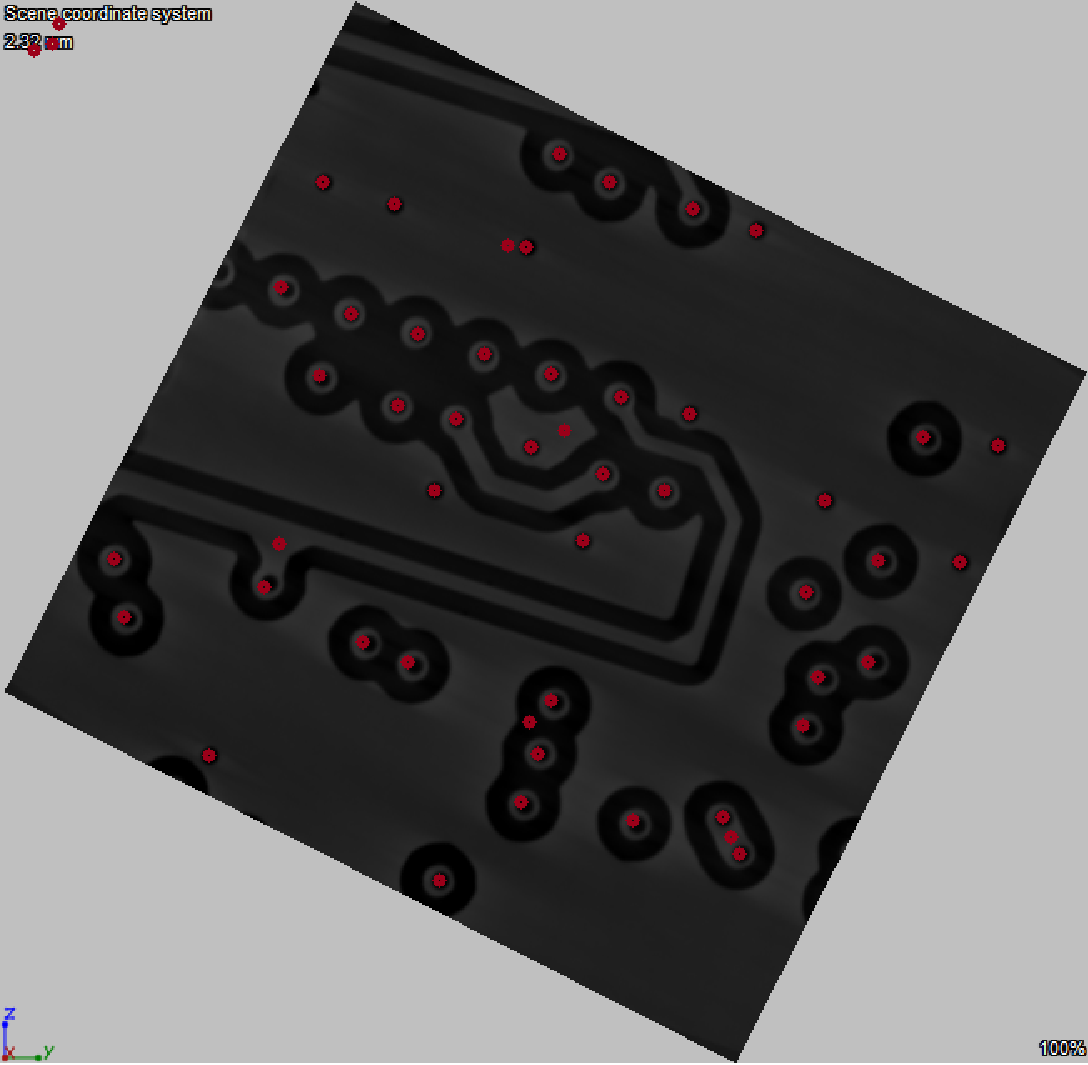
\includegraphics[width=0.8\textwidth]{matches2.pdf}
    \caption{Suchbild mit eingezeichneten gemergeten Merkmalsvektoren}
    \label{fig:suchbild_merge_matches}
  \end{center}
\end{figure}

Bis auf wenige Fehler in Form von Merkmalsvektoren, die keine Bohpunkte beschreiben, werden auf diese Art und Weise alle Bohrpunkte, egal ob mit oder ohne Isolierschicht, erkannt. \\
Dieses Verfahren eignet sich somit vor allem dann, wenn mehrere Unterschiedliche Bilder der gleichen Szene existieren (was in dem zu untersuchenden Bilderstack der Fall ist).
 

\section{Template Matching}
	Template Matching ist ein Verfahren, bei dem ein prototypisches Modell einer Struktur im Bild gesucht wird. Das Template ist dabei selbst ein kleines Bild, welches wie ein Filterkern über das Bild wandert.
\begin{figure}[H]
  \begin{center}
    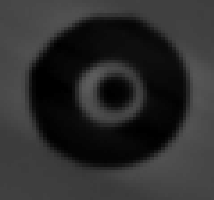
\includegraphics[width=0.6\textwidth]{template.pdf}
    \caption{Template eines Bohrpunktes (Vergrößert)}
    \label{fig:template}
  \end{center}
\end{figure}
Dabei wird in jedem Punkt $(x, y)$ ein Änhlichkeitsmaß des Templates gegenüber dem Bild berechnet.
Ein häufig verwendetes Änglichkeitsmaß ist dabei \textbf{Mean absolute difference (MAD)}.
Dieses Änhlichkeitsmaß bezeichnet die mittlere Differenz der Grauwerte des Bildes $g$ und des Templates $T$:
\begin{equation*}
MAD(x, y) = \frac{1}{M \cdot N} \sum_{ij}^{{}} \left | g(x +i, y + j) - T(i, j) \right |
\end{equation*}
Befindet sich bei der Suche das Template genau über der gesuchten Struktur, ist $MAD(x, y)$ minimal, während bei keiner Übereinstimmung des Templates und des Bildausschnittes $MAD(x, y)$ groß ist. Dadurch sind im resultierenden Bild, in dem das Änhlichkeitsmaß abgebildet wird, lokale Minima die Orte, in denen sich die Struktur des Templates befindet.
\begin{figure}[H]
  \begin{center}
    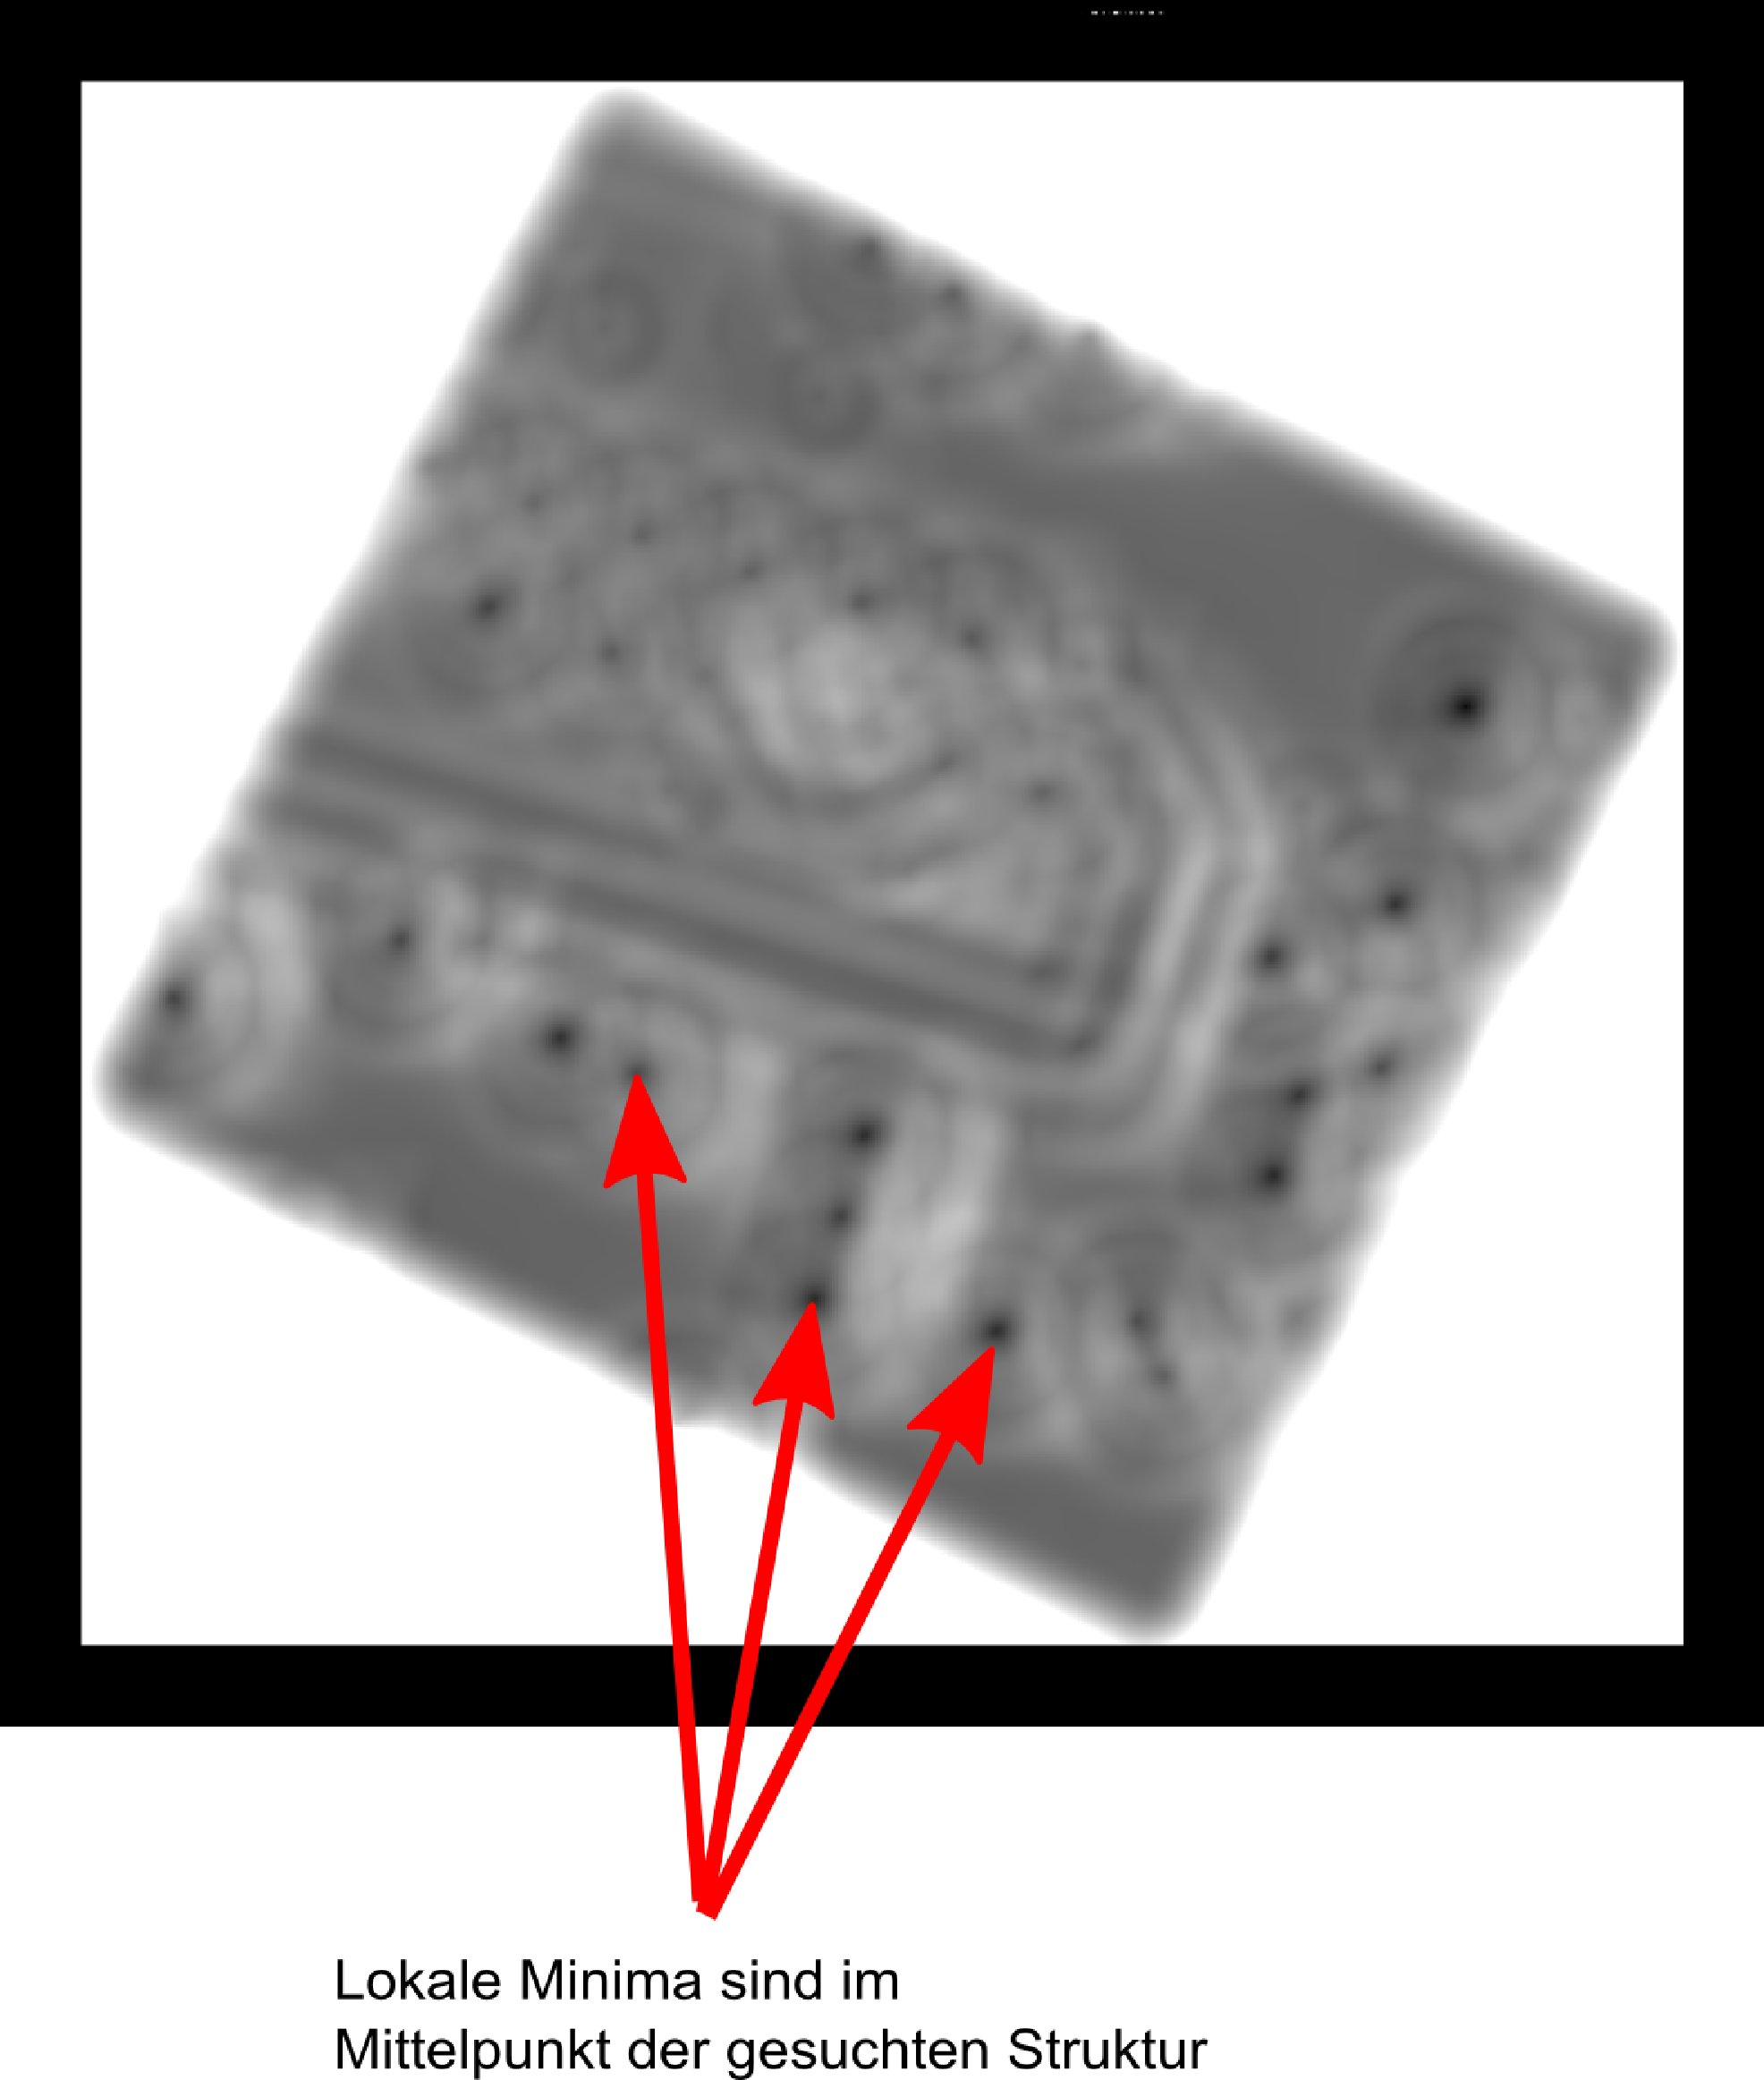
\includegraphics[width=0.7\textwidth]{loc_min.pdf}
    \caption{Lokale Minima}
    \label{fig:localminima}
  \end{center}
\end{figure}

\section{Einsatz der Houghtransformation zur Erkennung von Bohrpunkten}
Da gleichartige Bohrungen wohl auf der kompletten Platine den gleichen Radius (mit einer kleinen Toleranz) besitzen, kann auf 2d-Slices explizit nach Kreisen mit diesem Radius gesucht werden. Dies ergibt für Houghtransformation für Kreise mit Radius = 5 beispielsweise folgendes Bild im Akkumulatorraum:

\begin{figure}[H]
  \begin{center}
    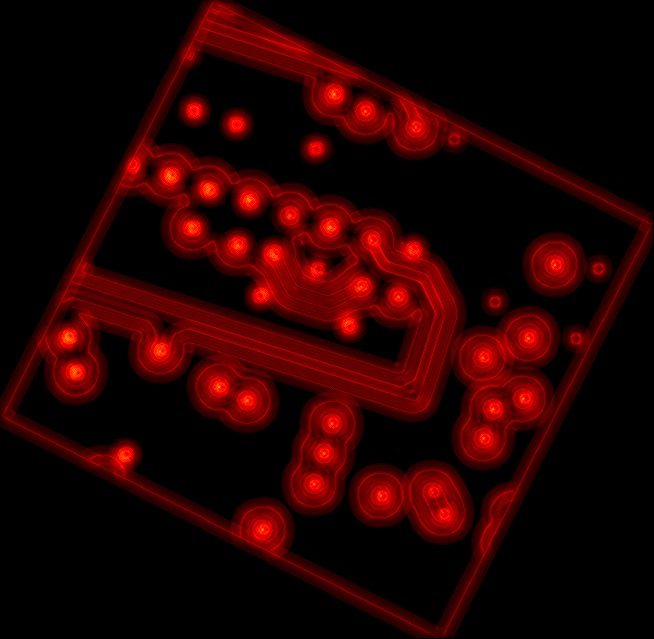
\includegraphics[width=0.7\textwidth]{houghkreiseakku.jpg}
    \caption{Akkumulatorraum für Kreise mit Radius = 5}
    \label{fig:houghkreiseakku}
  \end{center}
\end{figure}

Da die Radien jedoch leicht schwanken, was insbesondere durch die geringe Auflösung bedingt ist, kann beispielsweise noch der Raum für Kreise mit Radius 4 hinzuaddiert werden, um ein klareres Bild zu erhalten. 

\begin{figure}[H]
  \begin{center}
    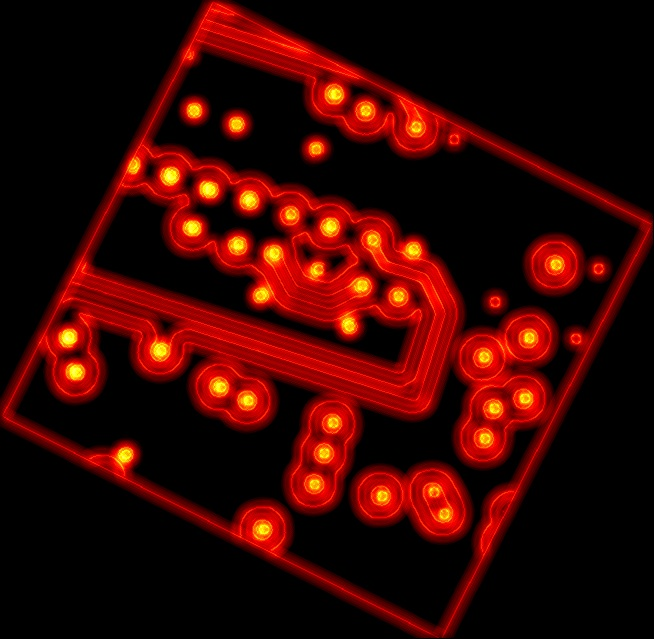
\includegraphics[width=0.7\textwidth]{houghkreiseakku2.jpg}
    \caption{Akkumulatorraum für Kreise mit r=4 und r=5}
    \label{fig:houghkreiseakku2}
  \end{center}
\end{figure}

In diesem Raum müssen nun die lokalen Maxima gefunden werden. Dies ist keine triviale Aufgabe, da ein lokales Maxima in einem anderen Bildbereich eher zum oberen Durchschnitt gehört. Es bietet sich hier der Einfachheit halber dennoch an, alle Pixel oberhalb eines Schwellwertes (z.B $0.6 \cdot globMax$) zu Clustern zusammenfassen und aus diesen jeweils den Mittelpunkt als Bohrung zu speichern. 

\begin{figure}[H]
  \begin{center}
    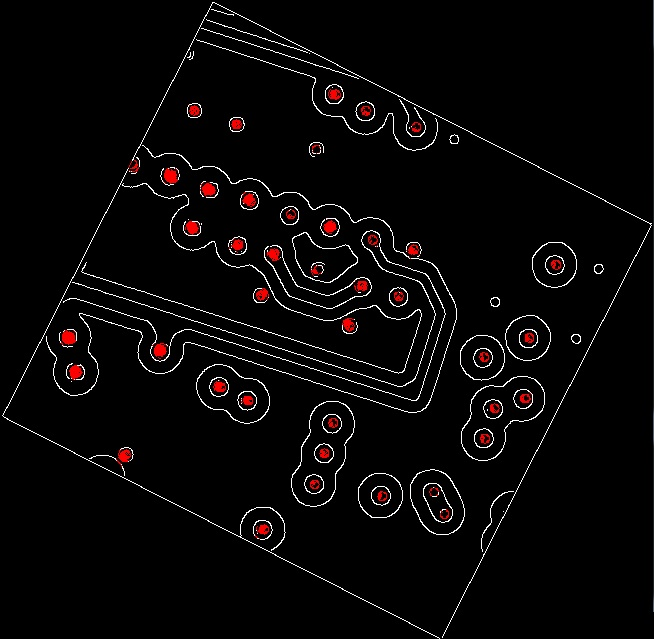
\includegraphics[width=\textwidth]{canny_HoughRes.jpg}
    \caption{Pixel mit höherem Wert als $0.6 \cdot globMax$}
    \label{fig:houghkreiseakku2}
  \end{center}
\end{figure}

Wendet man ein solches Schwellwertverfahren an, so müsste der Schwellwert heuristisch optimiert werden, um möglichst viele Punkte zu “erwischen”, da Bohrungen ohne umliegende Kanten (bspw. Isoliermaterial) generell schächer in den Akkumulatorraum abgebildet werden. \newline
Um dieses Bild zu verbessern, hat man natürlich die Möglichkeit den Akkumulatorraum mit verschiedenen Filtern zu falten, um damit bspw. alle kreisförmigen Maxima zu verstärken. \newline
Ansonsten könnte man beispielsweise verschiedene “Hill-Climbing”-Algorithmen einsetzen, wobei hier zu beachten ist, dass ein lokales Maximum nur dann als Hinweis für eine Bohrung interpretiert werden darf, wenn die Menge zusammenhängender, umgebender Pixel mit ähnlich hohem Wert lokal relativ beschränkt ist. Dadurch werden nur “punktförmige” Maxima gefunden.

\section{Alternativer Algorithmus zur Erkennung von Bohrpunkten auf Grundlage einer Färbung}
Die Houghtransformation für Kreise ist relativ rechenintensiv und schließlich muss der Akkumulatorraum noch ausgewertet werden. Auch das Templatematching arbeitet mit Filterkernen, die so groß sind wie die gesuchten Kreise. Dies motivierte dazu einen schnelleren Algorithmus zu entwickeln, zur Not auch auf Kosten der Universalität.
Eine sehr einfache und effiziente Möglichkeit Kreise in einem Canny-Edge Bild zu finden ist die folgende:
\newline
%\begin{Algorithmus}
%\caption{Algorithmus in Pseudocode}
%\label{alg:sample}
\begin{algorithmic}
\Procedure{FindHoles}{Bild $img$, Radius $r$, Toleranz $t$}
\ForAll{Pixel $p \in img$}
  \If{$p$ ist weiß}
    \State Folge der zugehörigen weißen Linie $l$ ungefähr $n$ Schritte lang
    \State , wobei $n <= int(2\cdot\pi\cdot(r+t))$
      \ForAll{Mittelpunkte $mp$}\Comment Geschätzt aus der Position von $p$.
        \If{$\exists lp \in l: dist(mp, lp) < r - t \lor dist(mp, lp) > r + t $}
          \State Abbrechen             
        \EndIf 
        \If{Die Linie umschließt den Mittelpunkt (z.B. Quadrantencheck)}
          \State l sei ein Kreis; continue in äußerer Schleife            
        \EndIf
      \EndFor
  \EndIf
\EndFor
\EndProcedure \newline
\end{algorithmic}
%\end{Algorithmus}

\begin{figure}[H]
  \begin{center}
    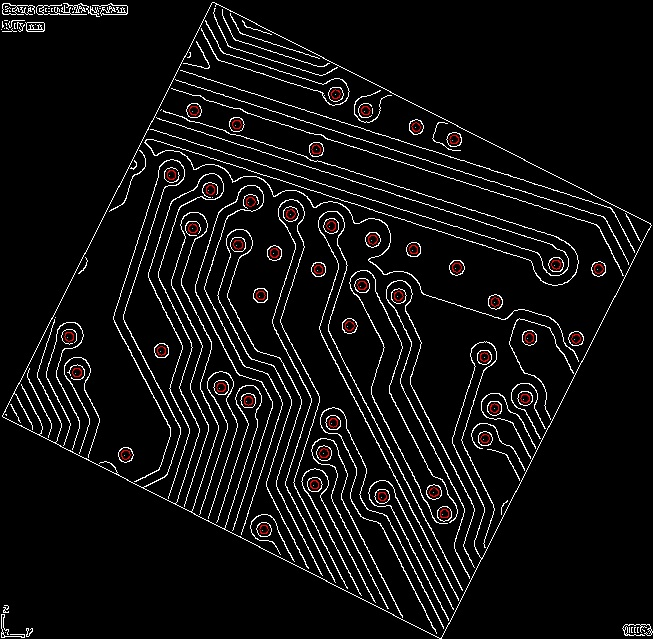
\includegraphics[width=\textwidth]{canny2_PA1.jpg}
    \caption{Ein Resultat des Algorithmus (gefundene Bohrungen sind rot markiert)}
    \label{fig:b_alg_1}
  \end{center}
\end{figure}


\subsection{Bewertung:}
Der Algorithmus ist extrem schnell und erkannte in sämtlichen Testbildern ohne Probleme alle gesuchten Kreise. Falls die Kantendetektion einen Fehler gemacht hat und der Kreis eine kleinere Lücke beinhaltet, so wird der Kreis im allgemeinen dennoch erkannt (Falls die Lücke nicht zu groß ist). \newline
Problematisch könnte selbstverständlich die Verallgemeinerung auf die gleichzeitige Suche von Kreisen beliebiger Radien werden. Diesbezüglich wurden noch keine Anstrengungen unternommen, da hierfür noch keine Notwendigkeit bestand.

\section{Einsatz der Houghtransformation zur Erkennung von Leiterbahnen}
Die Houghtransformation ist nicht direkt geeignet für das Erkennen von Leiterbahnen, da ausschließlich Geradenstücke erkannt werden. Aus Diesen lässt sich jedoch nicht schließen, ob es sich um eine Leiterbahn handelt oder nicht (es könnte z.B. auch Teil von Isoliermaterial sein). \newline
Die Kurven der Bahnen werden nicht erkannt, somit müsste man die Geradenstücke manuell verlinken und anschließend noch jeweils 2 Kanten (Bahnränder) zu einer Leiterbahn zusammenfassen. Zudem müssten andere, im Bild vorkommende Geraden ausgeschlossen werden. \newline
Dieses Anpassungsverfahren scheint also um relativ kompliziert zu sein, da es einfachere Wege gibt die Bahnen zu finden.  

\section{Alternativer Algorithmus zu Erkennung von Leiterbahnen auf Grundlage einer Färbung}
Bohrungen sind relativ einfach zu finden, weil es sich um einigermaßen simple geometrische Objekte handelt. Da alle Leiterbahnen schließlich in einer Bohrung enden, motiviert die Idee einen Algorithmus zu schreiben, der bei bereits erkannten Bohrungen prüft, ob eine Leiterbahn in sie mündet.\newline
Ein Beispiel für einen solchen Algorithmus wäre folgendes Verfahren: \newline
\begin{enumerate}
\item Man zeichne einen Kreis $k1$, dessen Radius etwas größer ist als der Abstand vom Mittelpunkt der Bohrung bis zum äußeren Ende der umgebenden Isolierschicht. \newline
Da die gefundenen Bohrpunkte nicht immer perfekt in der Mitte liegen, untersucht man auch die Umgebungen jedes Bohrpunktes.
\item Falls in diesem Kreis ausgenommen von “weiß” und “schwarz” nur zwei Farben vorkommen, so weiß man, dass es sich entweder um eine Bohrung mit Leiterbahn handelt, oder aus Versehen eine “fremde” Region geschnitten wurde. 
\item Betrachtet man das Vorkommen der selteneren Farbe in einem Kreis $k2$, dessen Radius etwas kleiner ist, als der Radius von $k1$, so kann man anhand eines einfachen Vergleichs des Mengenverhältnisses in $k1$ und $k2$ schätzen, dass es sich um ein Leiterbahn handeln kann. \newline
Dies liegt daran, dass die Farbe der Leiterbahn in beiden Kreisen in ungefähr gleich vielen Pixeln auftauchen muss (im inneren Kreis evtl. etwas häufiger).
\end{enumerate}

\begin{figure}[H]
  \begin{center}
    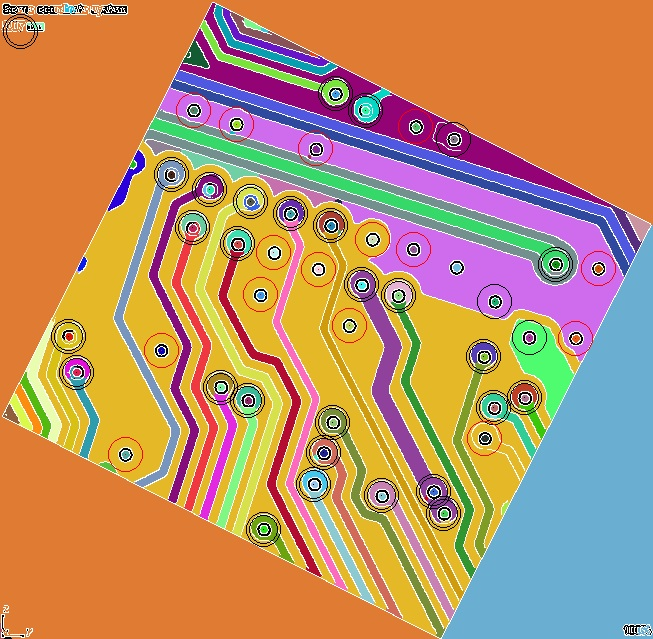
\includegraphics[width=\textwidth]{canny2_FACA1_test.jpg}
    \caption{Eingezeichnete Kreise (bei roten Kreisen ist bereits das Kriterium aus Schritt zwei verletzt.)}
    \label{fig:l_alg_1_test}
  \end{center}
\end{figure}

\begin{figure}[H]
  \begin{center}
    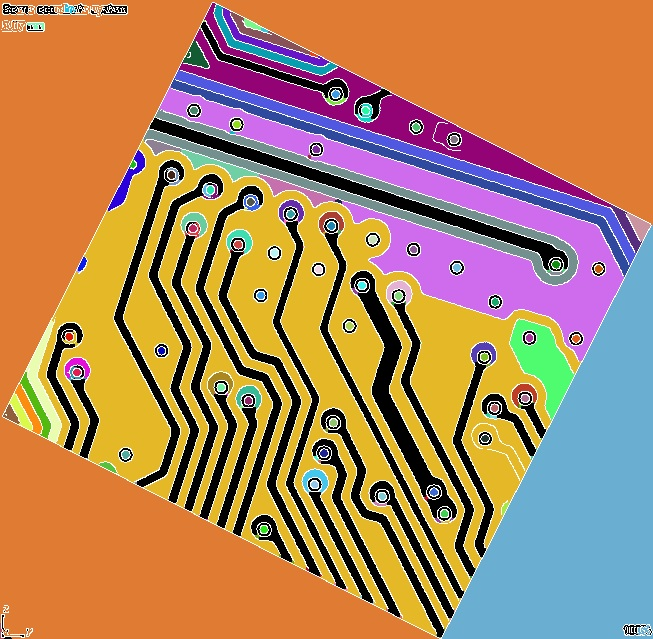
\includegraphics[width=\textwidth]{canny2_FACA1.jpg}
    \caption{Ein Resultat des Algorithmus (gefundene Leiterbahnen sind schwarz markiert)}
    \label{fig:l_alg_1}
  \end{center}
\end{figure}

\subsection{Bewertung:}
Der Algorithmus ist relativ schnell, da er nur die bereits gegebenen Bohrungen untersucht und nicht daher nicht das komplette Bild durchforstet. \newline
Gegenüber Fehlern im “Canny”-Bild ist der Algorihtmus nur insofern robust wie es der verwendete Färbealgorithmus ist. \newline
Problematisch ist natürlich auch hier, dass der Algorithmus speziell auf das Problem zugeschnitten wurde und daher an Universalität einbüßt.

\section{Weiterer alternativer Algorithmus zu Erkennung von Leiterbahnen}
Da der vorherige Algorithmus von Robustheit des Färbealgorithmus abhängt und daher im Allgemeinen anfällig ist für Fehler des Canny-Edge-Detektors, wäre ein Algorithmus interessant, welcher ohne Färbung auskommt. \newline
Da die Bohrungen bisher zuverlässig erkannt wurden und es das Verfahren extrem beschleunigt, soll auch hier wieder von den gefundenen Bohrungen ausgegangen werden. \newline
Der hier vorgeschlagene, auf das Problem abgestimmte Algorithmus sucht im Wesentlichen die Kante(n) einer eventuellen Leiterbahn und untersucht ihr Verhalten bezüglich der Umrundung des Bohrpunktes: \newline

\begin{enumerate}
\item Man zeichne wieder einen Kreis, dessen Radius etwas größer ist als der Abstand vom Mittelpunkt der Bohrung bis zum äußeren Ende der umgebenden Isolierschicht. \newline
Da die gefundenen Bohrpunkte nicht immer perfekt in der Mitte liegen, untersucht man auch die Umgebungen jedes Bohrpunktes.
\item Falls es auf dem Kreis genau zwei weiße Cluster gibt und deren euklidischer Abstand im Toleranzbereich der Breite einer Leiterbahn liegt, so kann man sagen, dass es sich entweder um die beiden Seiten der Leiterbahn handelt oder keine Leiterbahn von der Bohrung ausgeht und zufällig zwei fremde Punkte mit dem richtigen Abstand gefunden wurden.
\item Um letzteren Fall mit hoher Wahrscheinlichkeit auszuschließen könnte man beispielsweise jeweils der zugehörigen weißen Linie eines Clusters folgen und schließlich untersuchen, ob die Vereinigung der beiden Linien den Bohrpunkt umrundet (bspw. Quadrantencheck: Liegen in jedem Quadranten um den Bohrpunkt min. x Pixel?).
\end{enumerate}

\begin{figure}[H]
  \begin{center}
    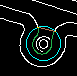
\includegraphics[width=0.7\textwidth]{CA1.png}
    \caption{Beispiel zu Verdeutlichung: Der in Schritt 1 gezeichnete Kreis ist blau; Die gefundenen Cluster sind gelb; Der gemessene Abstand ist braun; Die Vereinigung der beiden Linien grün.}
    \label{fig:l_alg_1}
  \end{center}
\end{figure}

Um nun die tatsächliche Leiterbahn zu extrahieren könnte man beispielsweise den Floodfill Algorithmus der braunen Linie im Bild starten und somit alle Pixel der Leiterbahn zu finden. Das würde jedoch dem Vorhaben widersprechen, ohne Färbung und der damit verbunden, bereits angesprochenen Schwäche auszukommen. \newline
Daher bietet es sich beispielsweise folgendes Verfahren zur Extraktion der Leiterbahnen an (Die Leiterbahnen machen keine scharfen Kurven): \newline

\begin{enumerate}
\item Man schießt einen Strahl, ausgehend vom Bohrpunkt in Richtung Leiterbahn, dh. durch die Mitte der gezeichneten, braunen Linie.
\item Der Strahl wird am Punkt p gestoppt, und zwar $n$ Pixel vor einer weißen Linie.
\item Anschließend vergleicht man $n$ mit $n_{links}$ und $n_{rechts}$, welche entstehen, wenn man, anstatt von p geradeaus zu gehen um um $45^\circ$ nach links bzw. nach rechts geht. 
\item Den längsten der drei Wege wählt man als neuen Startweg, halbiert den Winkel und macht weiter bei Schritt 3. Durch diesen Trick wird bei den Leiterbahnen für jeden aktuellen Punkt p der längste Weg in die richtige Richtung gefunden (siehe nachfolgende Grafik).
\item Wenn man den längsten Strahl ausgehend vom Punkt p gefunden hat, dann wird p neu gesetzt, indem man mit diesem Strahl wieder bei Schritt 2 weitermacht. Falls kein neuer Strahl gefunden wurde ist man fertig.
\end{enumerate}

\begin{figure}[H]
  \begin{center}
    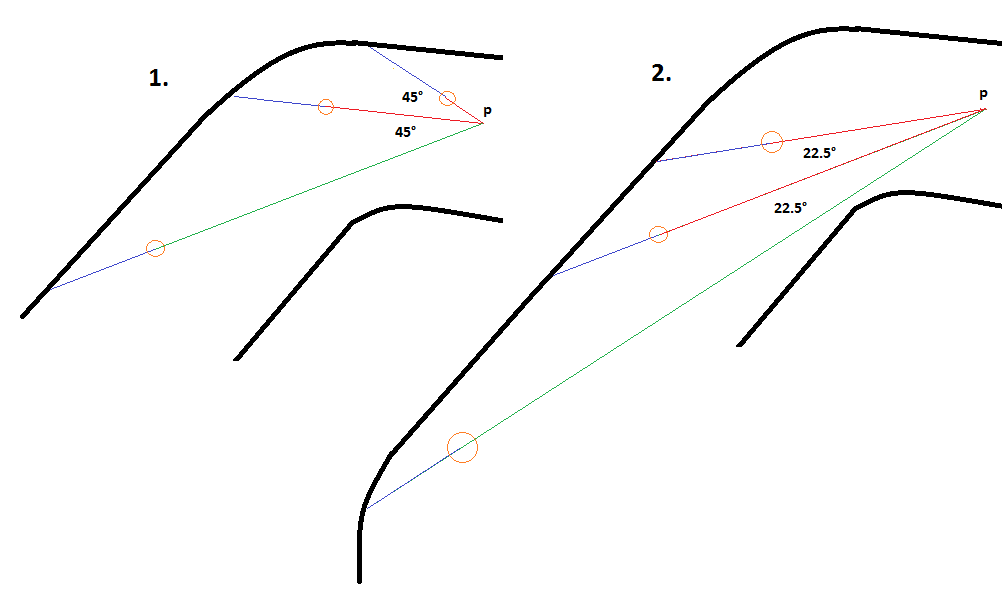
\includegraphics[width=0.7\textwidth]{LinienpunkteMuster.png}
    \caption{Zwei Iterationsschritte zu Verdeutlichung: Der grüne Weg ist jeweils der längste und wird daher als Ausgangsrichtung für die nächste Winkelhalbierung gesetzt.}
    \label{fig:linepoints}
  \end{center}
\end{figure}

Dieses Vorgehen führt dazu, kleinere Lücken im Kantenbild mit einigermaßen hoher Wahrscheinlichkeit übersprungen werden, insbesondere dann, wenn sie auf einem langen, geradlinigen Abschnitt auftauchen. Dieser Vorteil ist im folgenden Bild zu sehen, in welchem auch die Leiterbahn gefunden wurde, welche beim vorherigen Verfahren aufgrund der fehlerhaften Färbung nicht erkannt wurde.

\begin{figure}[H]
  \begin{center}
    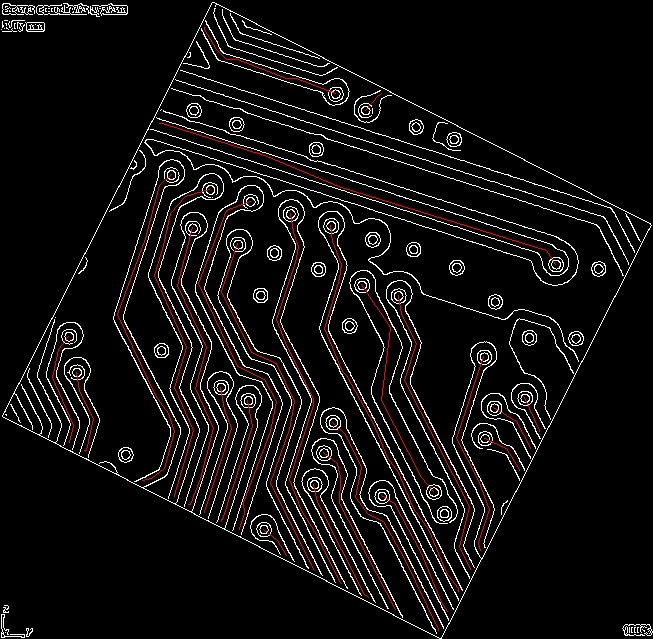
\includegraphics[width=\textwidth]{canny2_CA1_Circuits.jpg}
    \caption{Ein Resultat des Algorithmus (gefundene Leiterbahnen sind rot markiert). Es wurden zusätzlich Leiterbahnen, welche zwischen zwei Bohrungen verlaufen kombiniert.}
    \label{fig:linepoints2}
  \end{center}
\end{figure}

\begin{figure}[H]
  \begin{center}
    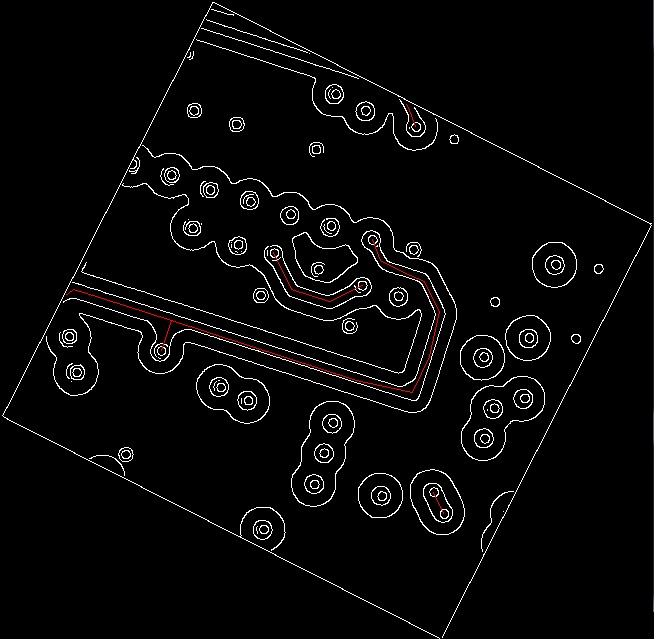
\includegraphics[width=\textwidth]{canny_CA1_Circuits.jpg}
    \caption{Ein anderes Resultat des Algorithmus (gefundene Leiterbahnen sind rot markiert). Außerdem wurden Leiterbahnen, welche zwischen n Bohrungen verlaufen zu einem Graph kombiniert.}
    \label{fig:linepoints22}
  \end{center}
\end{figure}

\subsection{Bewertung:}
Durch die beidseitige Verfolgung der von den Clustern ausgehenden Linien und dem anschließenden Check deren Vereinigung bezüglich dem Quadrantenkriterium hat sich das Verfahren für die Erkennung von Leiterbahnen auch bei Lücken im Canny-Edge-Bild bewährt. \newline
Das Verfahren zur nachfolgenden Extraktion der Leiterbahnen hat in den getesteten Szenarien gut funktioniert und ist einigermaßen einfach zu implementieren. \newline
Wenn ein Strahl jedoch zufällig durch eine Lücke im Kantenbild springt, dann hat das unabsehbare Konsequenzen und die Leiterbahn muss aus der Liste gestrichen werden. Ersteres ist wiederum einem Algorithmus nicht auf trivialem Wege ersichtlich und diesbezüglich müssen weitere Anstrengungen unternommen werden. \newline
Auch dieser Algorithmus ist extrem schnell und dürfte keinerlei Performanz-Probleme bereiten. 